% id: 0225
% book: RPM 중3-2 수학 · 02 삼각비의 활용
% section: 중단원 마무리하기
% figure: crop:fig-0225.png
% answer: ②
% answer_source: 답지
% variant_level: 0 (원본 전사)
% 이 파일은 build.mjs 가 items.json 에서 만든다. 고칠 때는 items.json 을 고친다.
\noindent\begin{minipage}[t]{0.58\linewidth}\vspace{0pt}\raggedright 오른쪽 그림과 같은 직각삼각형~$\pt{ABC}$에서 $\angle\pt{B}=37^\circ$, $\seg{AB}=10$일 때, $\triangle\pt{ABC}$의 둘레의 길이는? (단, $\sin 37^\circ=0.6$, $\cos 37^\circ=0.8$로 계산한다.)\end{minipage}\hfill\begin{minipage}[t]{0.4\linewidth}\vspace{0pt}\centering \setlength{\dmfigw}{76.4pt}\ifdim\dmfigw>\linewidth\setlength{\dmfigw}{\linewidth}\fi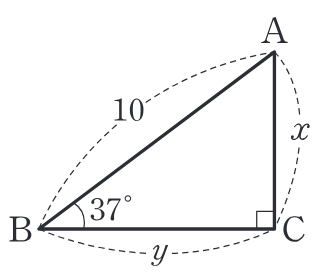
\includegraphics[width=\dmfigw]{figures/fig-0225.png}\end{minipage}\par
\dmchoicesauto{}{$23$}{$24$}{$25$}{$26$}{$27$}
